\begin{frame}{Previous Efficiency Studies : Overlay}
	\begin{figure}
		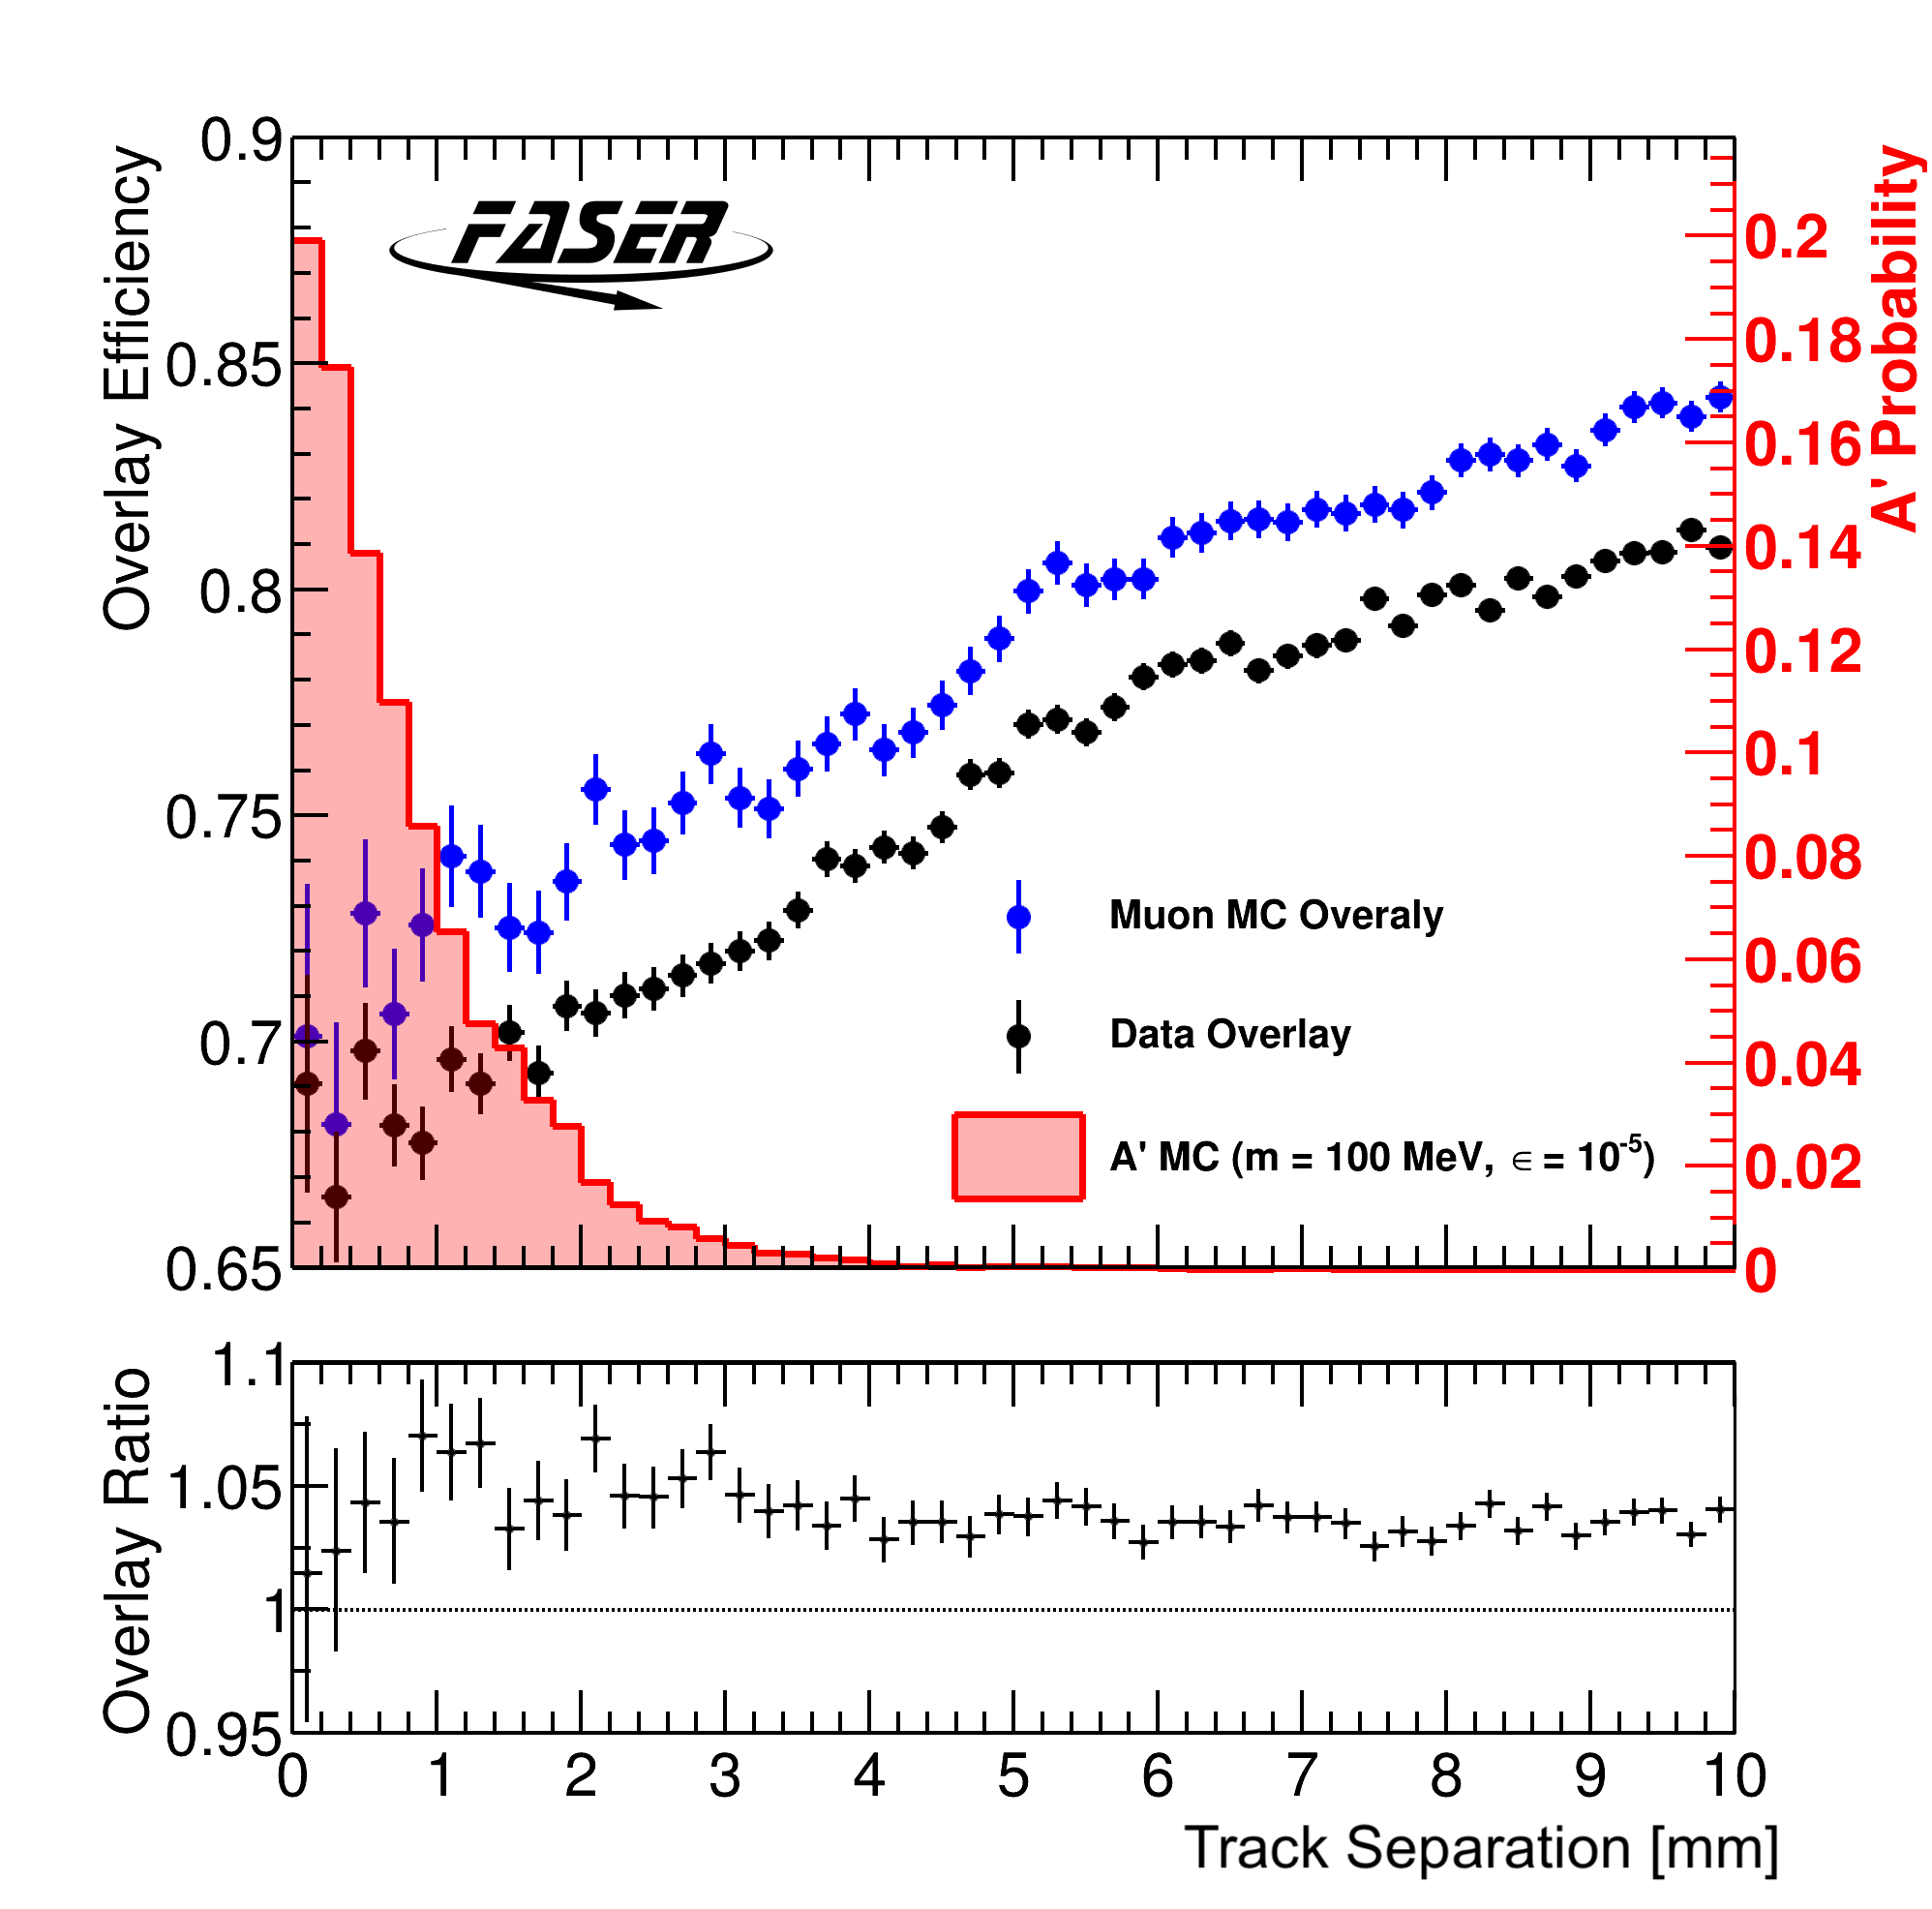
\includegraphics[height=0.7 \textheight]{./assets/OverlayTracks.png}
        \caption{ Overlay plot from \href{https://cds.cern.ch/record/2864686/plots}{Search for dark photons with the FASER detector at the LHC}\\ The separation variable used is the ``distance between the two tracks at their first measurements''}
	\end{figure}
\end{frame}

\begin{frame}{Previous Efficiency Studies : A' Tracking CutFlow}
    \begin{table}[h]
        \centering
        \resizebox{\linewidth}{!}{ 
            \begin{tabular}{lccccccccc}
                \toprule
                \multirow{2}{*}{Selection} & \multicolumn{4}{c}{ALMA9} & \multicolumn{4}{c}{CENTOS7} & \multirow{2}{*}{$\Delta$Eff.} \\
                \cmidrule(lr){2-5} \cmidrule(lr){6-9}
                & Pass & All & Eff. & Cum. Eff.
                & Pass & All & Eff. & Cum. Eff. \\
                \midrule
                $\geq$1 LongTracks & 56989 & 60000 & 94.98 & 94.98  & 56002 & 60000 & 93.34 & 93.34 & 1.64 \\
                $\geq$2 LongTracks & 46416 & 56989 & 81.45 & 77.36  & 45210 & 56002 & 80.73 & 75.35 & 0.72 \\
                 =2 LongTracks & 37807 & 46416 & 81.45 & 63.01  & 36746 & 45210 & 81.28 & 61.24 & 0.17 \\
                 \textcolor{red}{\textbf{Opposite Charge}} & 32427 & 37807 & 85.77 & 54.04  & 30375 & 36746 & 82.66 & 50.62 & \textcolor{red}{\textbf{3.11}}\\
                MaxRadius $<$ 100 & 31489 & 32427 & 97.11 & 52.48  & 29520 & 30375 & 97.19 & 49.20 & -0.08 \\
                \midrule
                \multicolumn{10}{c}{goodTrack Cuts}\\
                \midrule
                $\geq$ 7 Layers & 31435 & 31489 & 99.83  & 52.39  & 29472 & 29520 & 99.84  & 49.12 & -0.01 \\
                \textcolor{red}{\textbf{$\chi^2$/DoF $<$ 25}} & 31121 & 31435 & 99.00  & 51.87  & 27710 & 29472 & 94.02  & 46.18& \textcolor{red}{\textbf{4.98}} \\
                $\geq$ 7 DoF & 31115 & 31121 & 99.98  & 51.86    & 27706 & 27710 & 99.99  & 46.18 & -0.01\\
                \bottomrule
            \end{tabular}
        }
        \caption{Comparison of efficiency and cumulative efficiency for ALMA9 and CENTOS7.\\Note: The Cutflow is at an Event Level (not track level), thus the conditions have to met by all tracks in the event.}
        \label{tab:efficiency_comparison}
    \end{table}
    \begin{itemize}
        \scriptsize
        \item Highest improvement in goodTrack Cut of $\chi^2$/DoF $<$ 25
        \item Better ChargeID in ALMA9?
        \item We want to take a look at it differentially
    \end{itemize}
    
    \end{frame}


% \begin{frame}{Definition of Efficiency}
%     \textbf{General Idea}
% 	\begin{itemize}

%         \item One Track $\implies$ NOT reconstructed
%         \item Two Tracks with opposite charges $\implies$ Reconstructed 
%         \item More than two track $\implies$ Complicated
%     \end{itemize}
%     \vspace{1 cm}
%     \textbf{Potential Efficiency Metrics}
%     \begin{itemize}
%         \item Number of Events with $\geq$ 2 longTracks [good proxy]
%         \item MC Based Effi. [Using reconstructed-truth level data]
%     \end{itemize}
% \end{frame}

\begin{frame}{Definition of Fiducial}
    Before we define the efficiency we must account for the detector acceptance by ensuring the particle to be Fiducial.

    \vspace{0.5cm}
		% \textbf{Fiducial Criteria Based on Reconstructed Data}
		% \begin{itemize}
		% 	\item Requires $longTracks == 2$ 
		% 	\item $Track\_r\_atMaxRadius < 100$
		% 	\item $Track\_r\_at... < 100$
 		% \end{itemize}
		\textbf{Fiducial Criteria Based on Truth-Level Data}
		\begin{itemize}
			\item truthd0\_r [\{1,2,3\}] $<$ 100
			\item truthd1\_r [\{1,2,3\}] $<$ 100
			\item truthd0\_pz $>$ 20 GeV
			\item truthd1\_pz $>$ 20 GeV	
		\end{itemize}

        \vspace{0.3cm}
        {\small
        A truth-level prescription is preferred because the reconstruction-based approach depends on reconstruction performance, whereas ``fiducial'' should ideally be a function of the detector alone.}

        \vspace{0.2cm}

        {\scriptsize
            \textbf{Note:} truthd0\_r = $\sqrt{\text{truthd0\_x}^2 + \text{truthd0\_y}^2}$, and similarly for d1.

            % The p\_z cut is to ensure the particles don't stray too far from the LOS?
        }
\end{frame}


\begin{frame}{Fiducial CutFlow}
    \begin{table}[h!]
        \centering
        \small
        \begin{tabular}{lcccc}
            \toprule
            \textbf{Selection Criteria} & \textbf{Pass} & \textbf{All} & \textbf{Eff (\%)} & \textbf{Cum. Eff (\%)} \\
            \midrule
            truthd\_st1\_r $<$ 100    & 59228 & 60000 & 98.71  & 98.71 \\
            truthd\_st2\_r $<$ 100    & 56549 & 59228 & 95.48  & 94.25 \\
            truthd\_st3\_r $<$ 100    & 52640 & 56549 & 93.09  & 87.73 \\
            truthd\_pz $>$ 20 GeV       & 50444 & 52640 & 95.83  & 84.07 \\
            % truthd_P > 20000: pass=50444      all=52640      -- eff=95.83 % cumulative eff=84.07 %

            % truthd\_st1\_r $<$ 95     & 50316 & 52640 & 95.59  & 83.86 \\
            % truthd\_st2\_r $<$ 95     & 49866 & 50316 & 99.11  & 83.11 \\
            % truthd\_st3\_r $<$ 95     & 48217 & 49866 & 96.69  & 80.36 \\
            % truthd\_st1\_r $<$ 90     & 45882 & 48217 & 95.16  & 76.47 \\
            % truthd\_st2\_r $<$ 90     & 45453 & 45882 & 99.06  & 75.75 \\
            % truthd\_st3\_r $<$ 90     & 44037 & 45453 & 96.88  & 73.39 \\
            \bottomrule
        \end{tabular}
        
        \caption{Efficiencies and cumulative efficiencies for truth-level selection steps. [same for ALMA9/CENTOS7]}
        \label{table:truth_efficiency}
    \end{table}
    % \begin{lstlisting}
    %     truthd\_st1\_r = \\
    %     \hspace{0.5cm}sqrt( pow(truthd0\_x[1],2) + pow(truthd0\_y[1],2) ) $>$ 100 \&\& \\
    %     \hspace{0.5cm}sqrt( pow(truthd1\_x[1],2) + pow(truthd1\_y[1],2) )
    % \end{lstlisting}
\end{frame}

\begin{frame}{Track Reconstruction Efficiency Defined}
    \begin{itemize}
        \item Remove acceptance based on fiducial cuts at truth level
        \item Define Efficiency as the fraction of events with $\geq$2 reconstructed longTracks divided by the total number of events which is same as $\geq$0 longTracks. [Given both are fiducial] 
        \[ \text{Efficiency} = \frac{\text{NEvents}({\geq 2 \text{longTracks}}\ | \ \text{fiducial})}{\text{NEvents}(\geq0{\text{longTracks}}\ | \ \text{fiducial})} \]
    \end{itemize}
\end{frame}

\begin{frame}{$\geq2$ Track Efficiency as a function of DeltaR1}
    \begin{figure}
        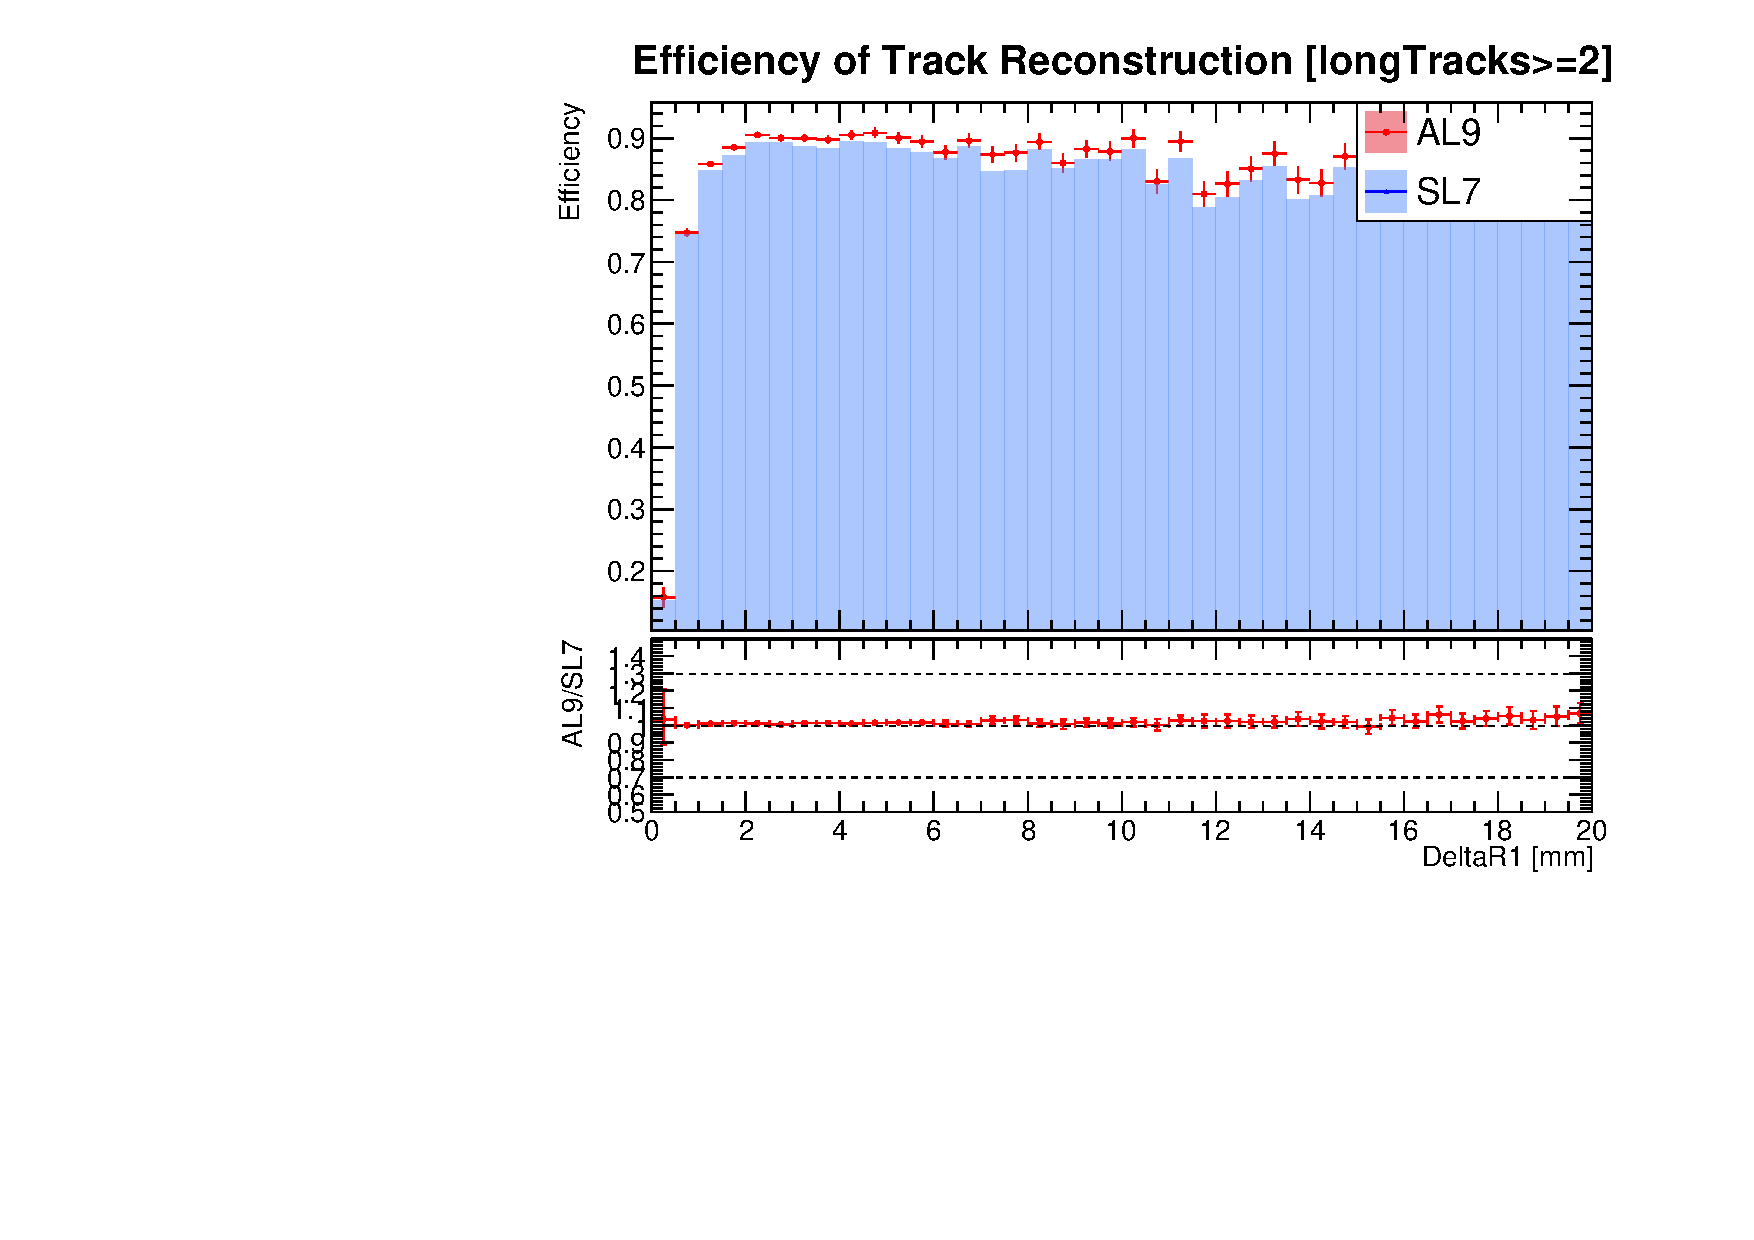
\includegraphics[width=0.7\linewidth]{./output/Effi_greq2_DeltaR1.pdf}
    \end{figure}
    \begin{itemize}
        \item There is generally agreement between ALMA9 and CENTOS7
        \item Although characteristics is different from the overlay study
        \begin{itemize}
            \item Overlay shows a more gradual growth to 90\% efficiency
        \end{itemize}
    \end{itemize}
\end{frame}

\begin{frame}{$\geq2$ Track Efficiency as a function of DeltaR1}
    \begin{figure}
        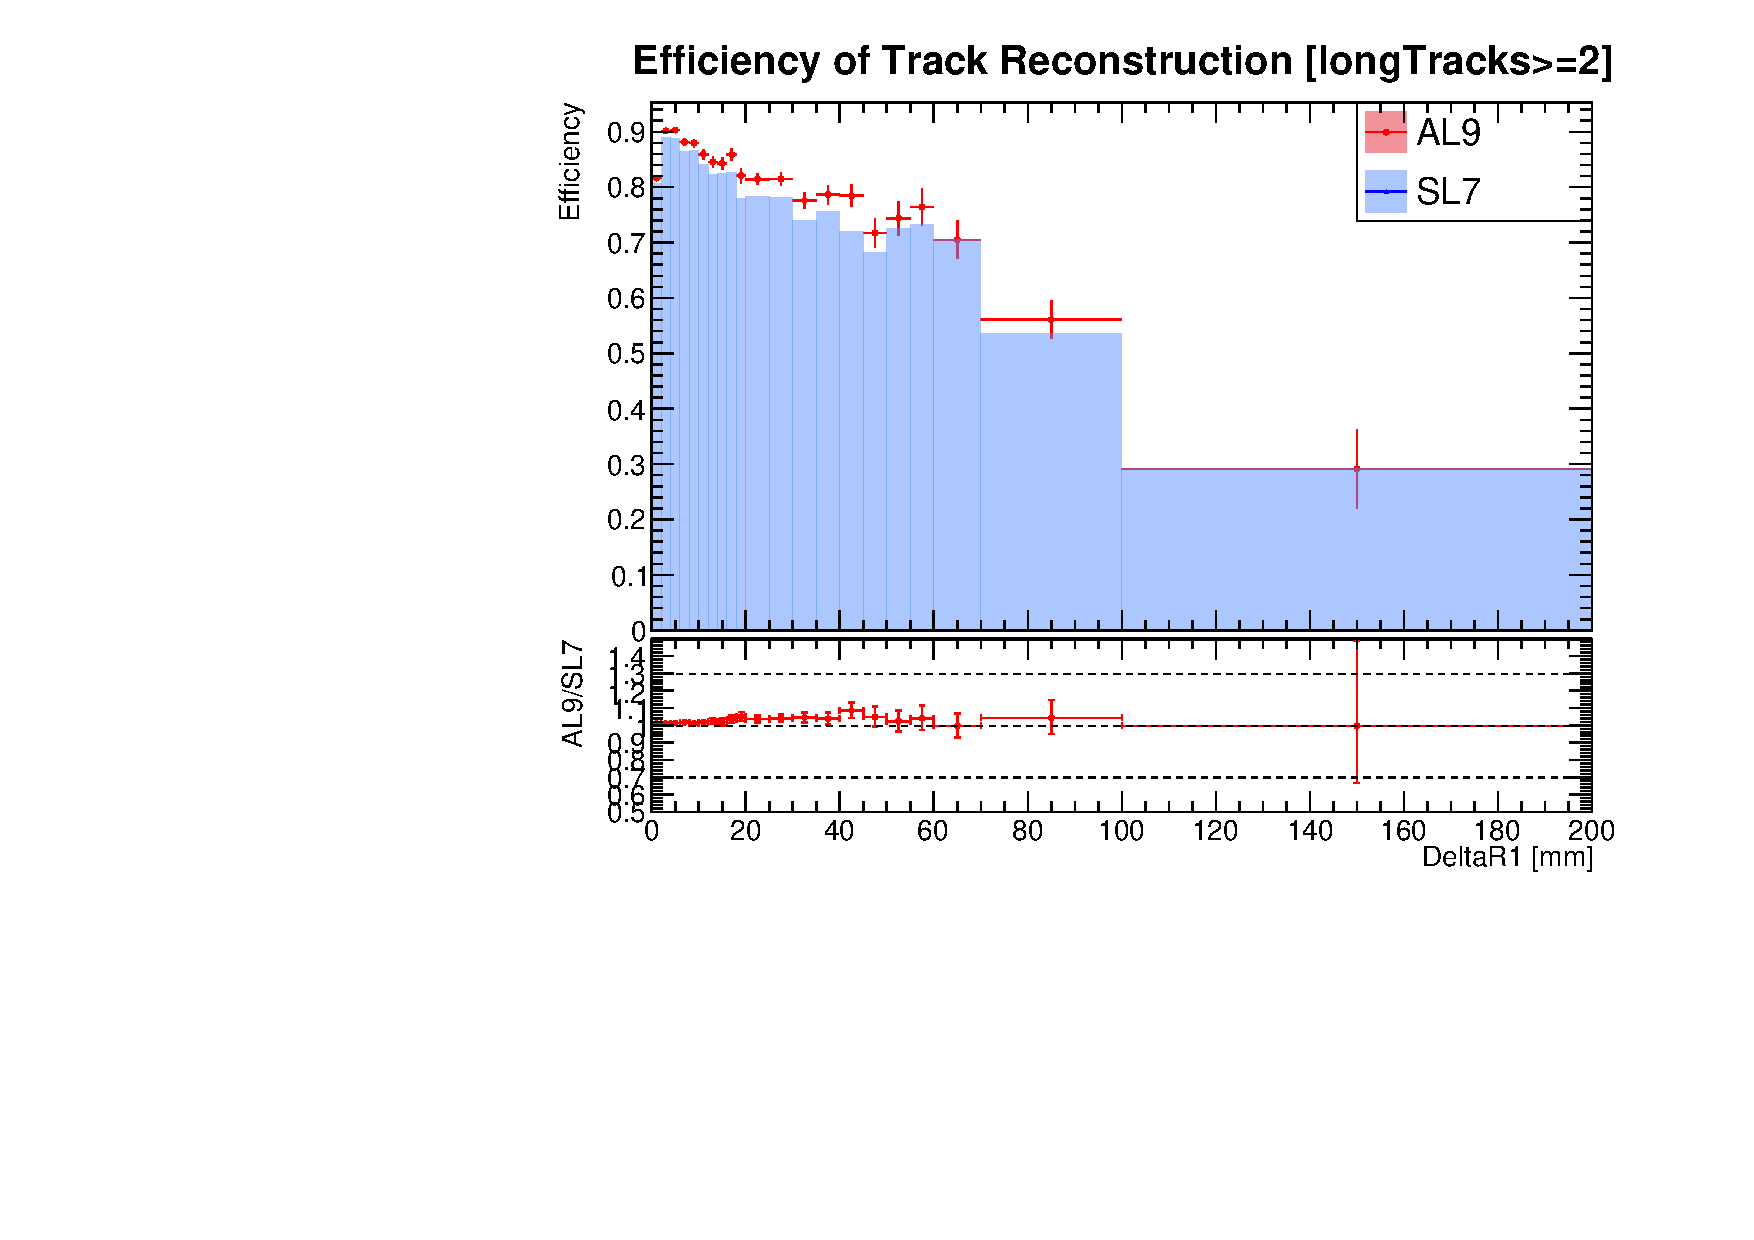
\includegraphics[width=0.8\linewidth]{./output/Effi_greq2_DeltaR1_unzoom.pdf}
    \end{figure}
    \begin{itemize}
        \item The Efficiency seem to decay at higher separation!
    \end{itemize}
\end{frame}

\begin{frame}{$\geq2$ Track Efficiency as a function of Theta1}
    \begin{figure}
        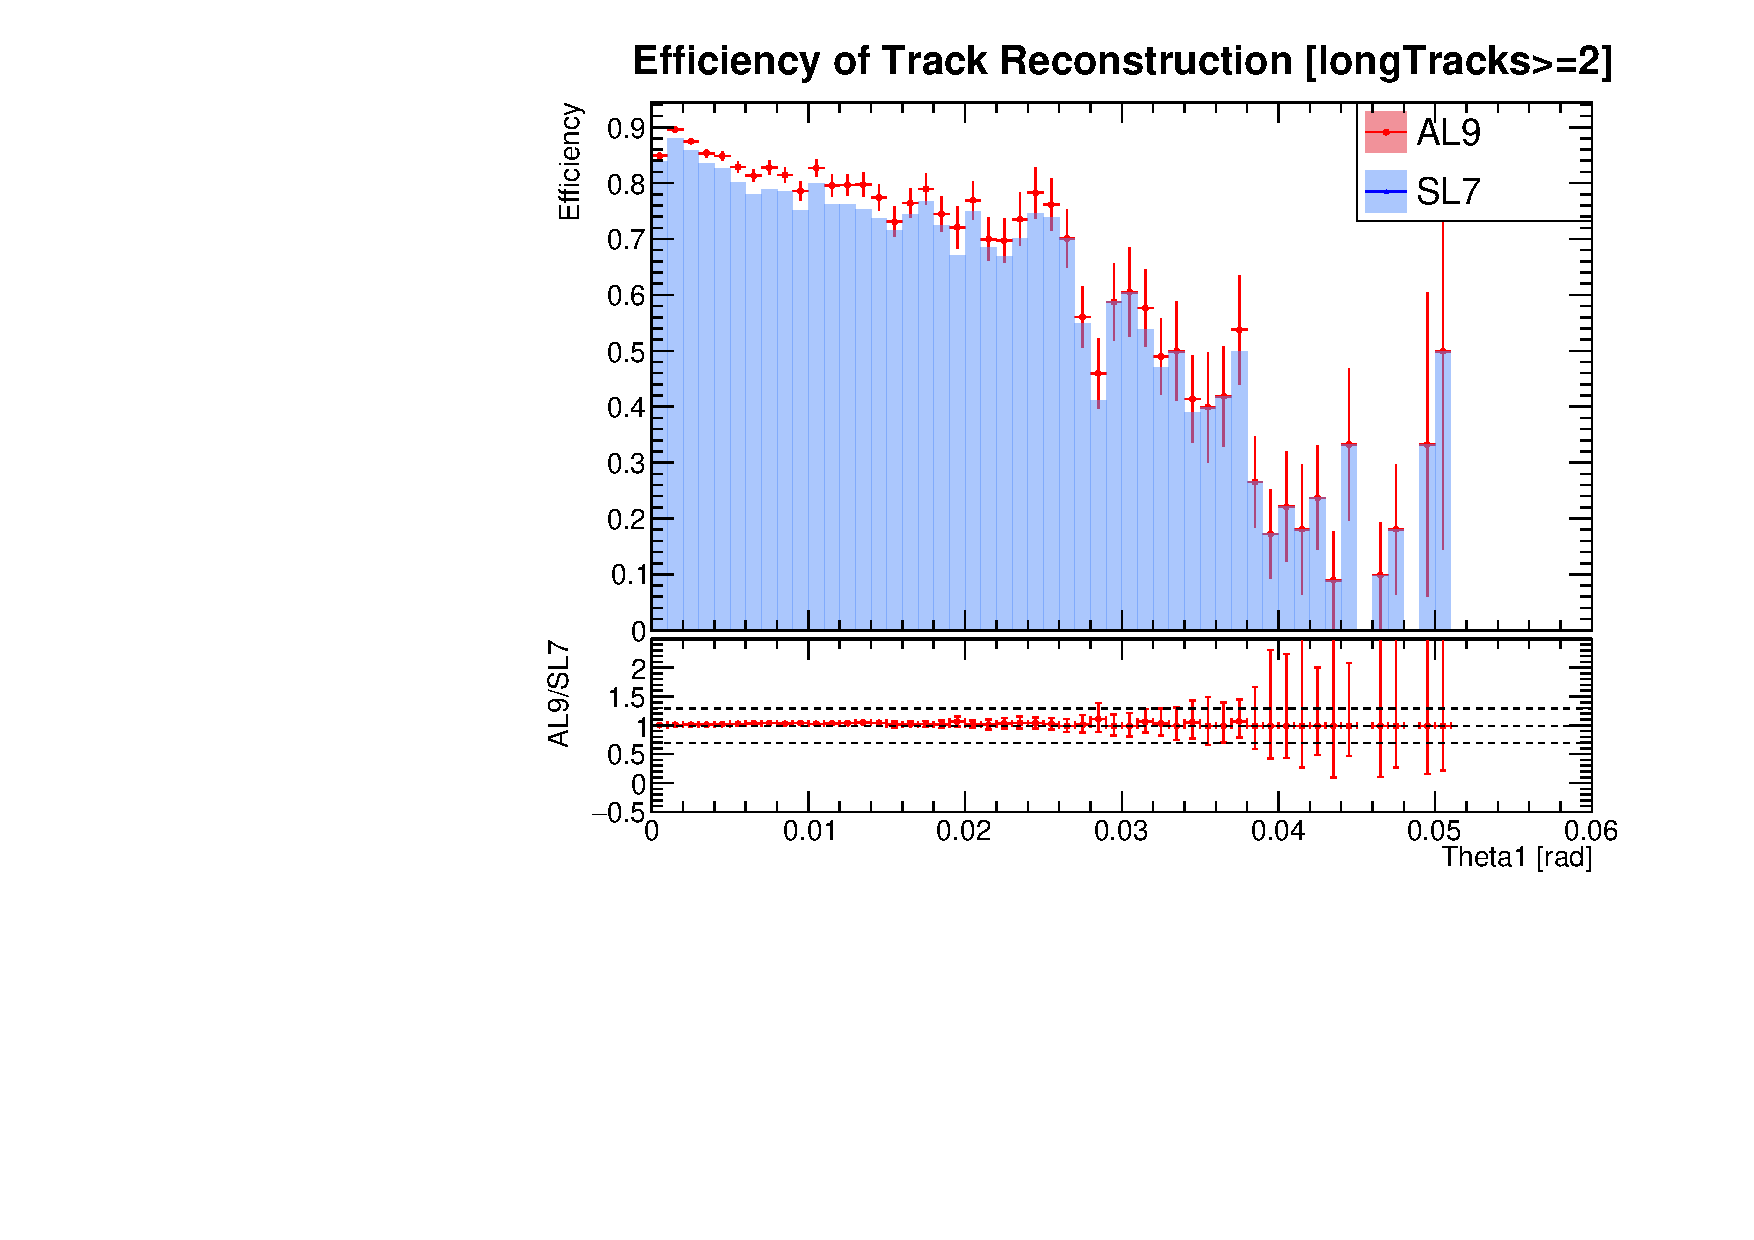
\includegraphics[width=0.8\linewidth]{./output/Effi_greq2_Theta1.pdf}
    \end{figure}
    \begin{itemize}
        \item The decay of efficiency at large separation is existent here as well.
    \end{itemize}
\end{frame}

% \begin{frame}{$\geq2$ Track Efficiency as a function of DeltaRP}
%     \begin{figure}
%         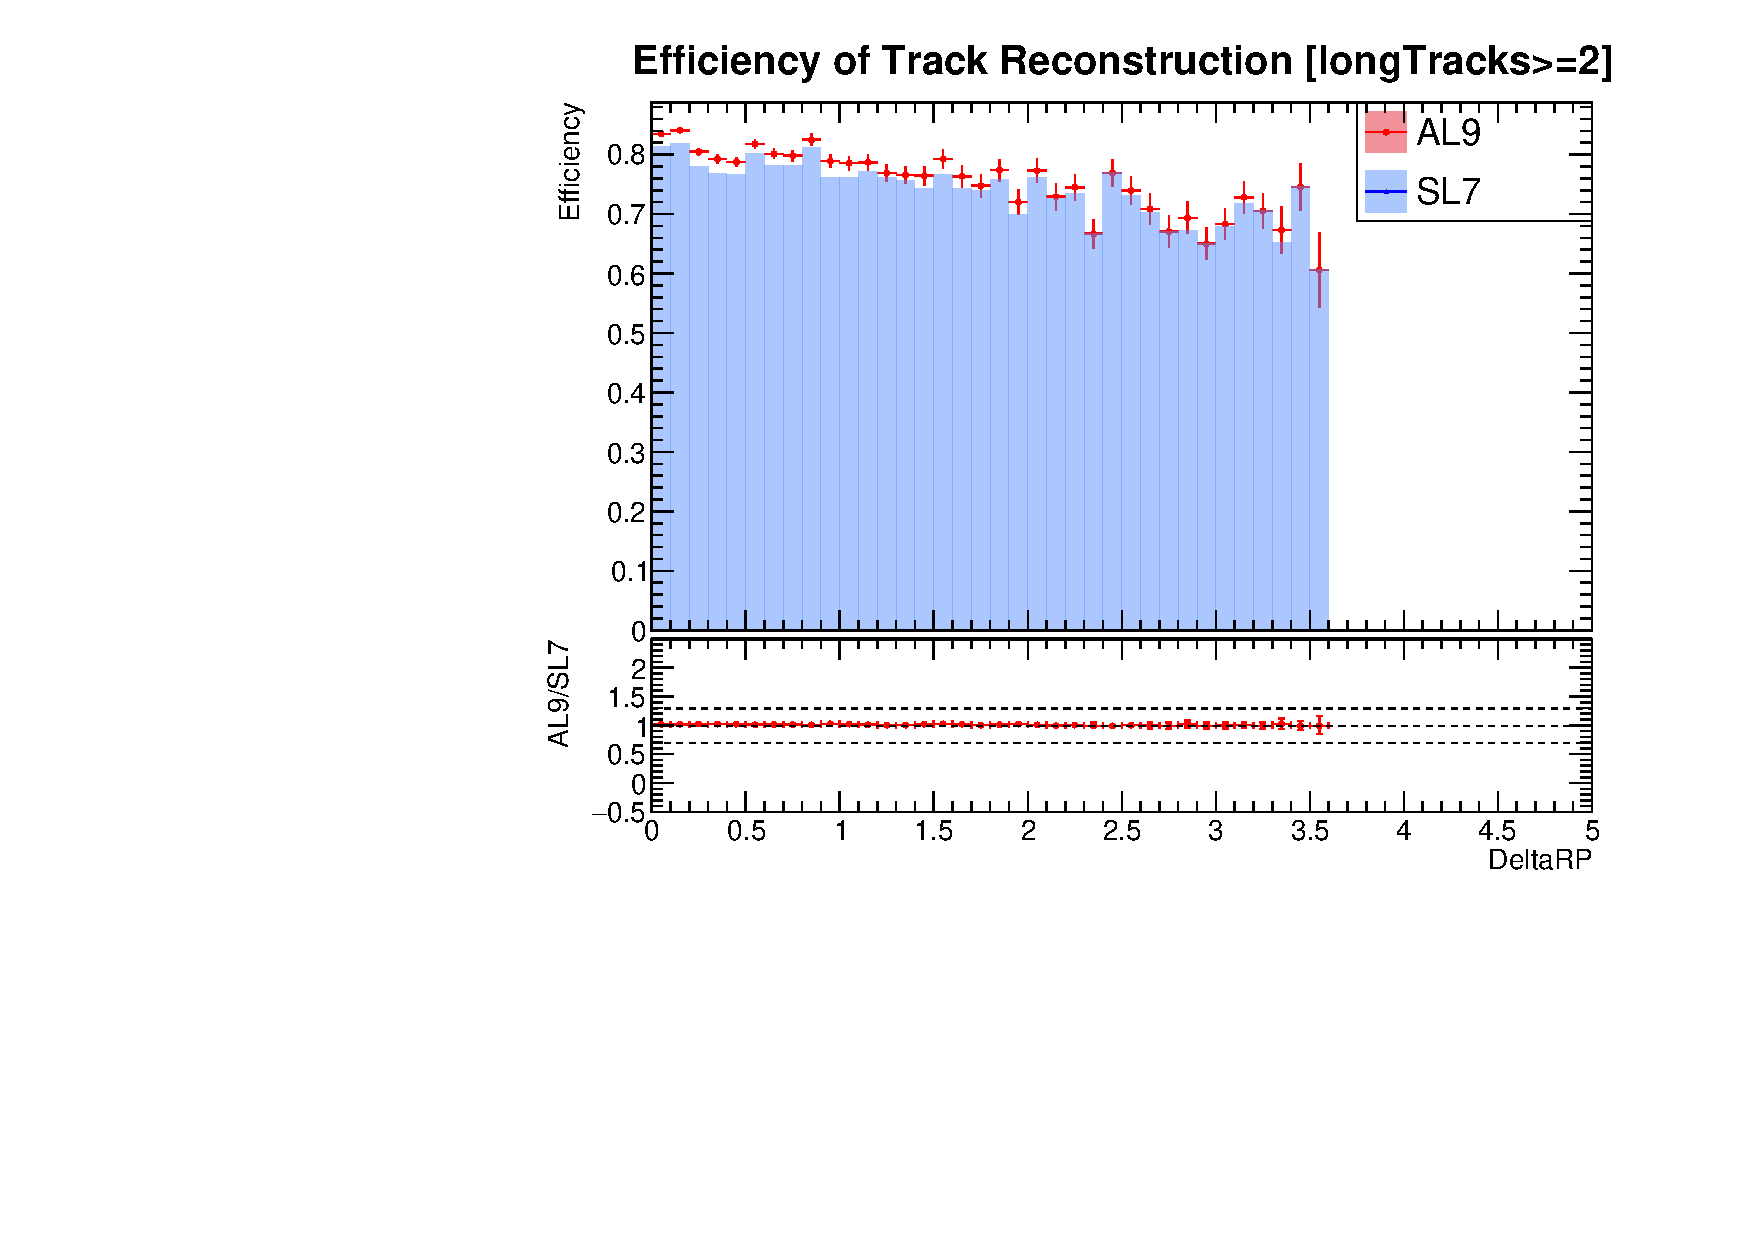
\includegraphics[width=\linewidth]{./output/Effi_greq2_DeltaRP.pdf}
%     \end{figure}
% \end{frame}

\begin{frame}{Efficiencies as a Function of Separation @ Station 1}
    \begin{columns}
        \begin{column}{0.6\linewidth}
            \begin{figure}
                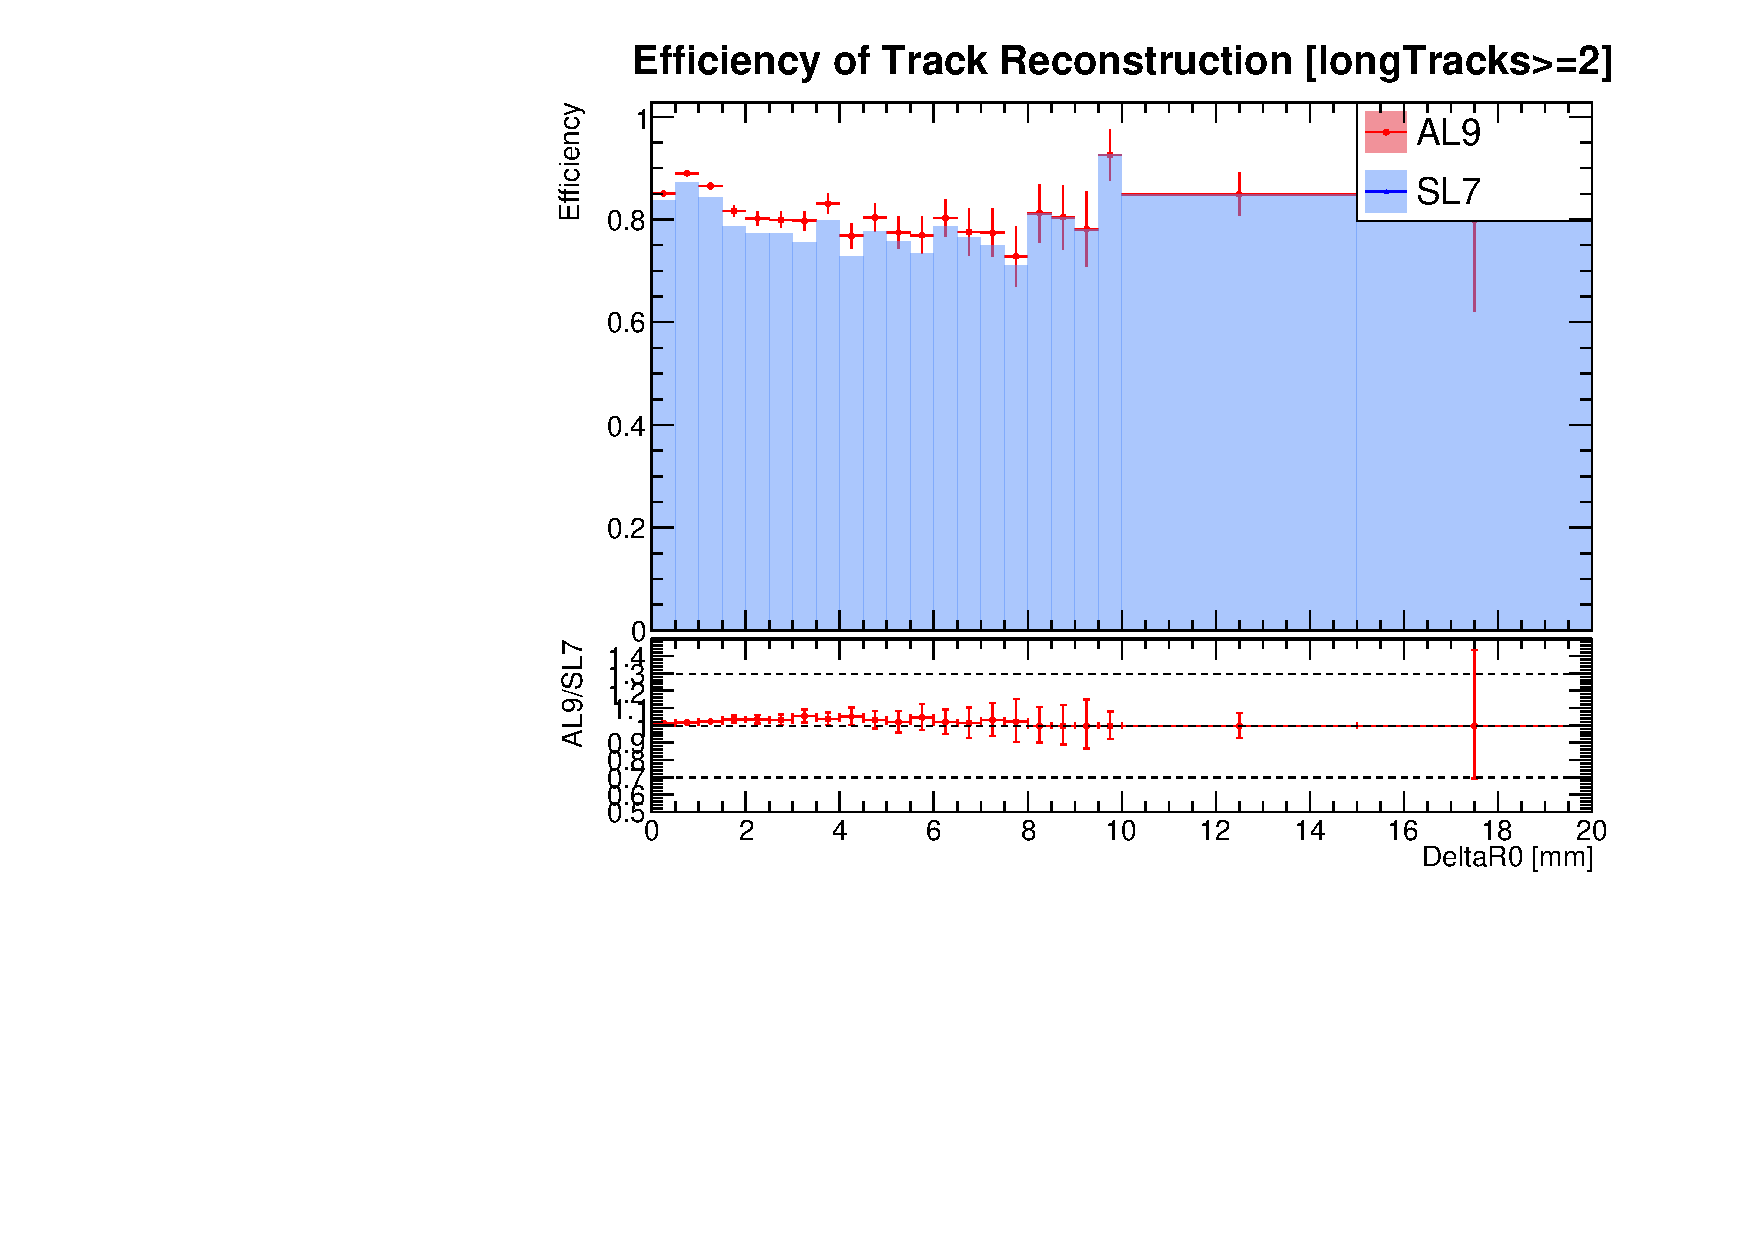
\includegraphics[width=1\linewidth]{./output/Effi_greq2_DeltaR0_unzoom.pdf}
            \end{figure}
        \end{column}
        \begin{column}{0.6\linewidth}
            \begin{figure}
                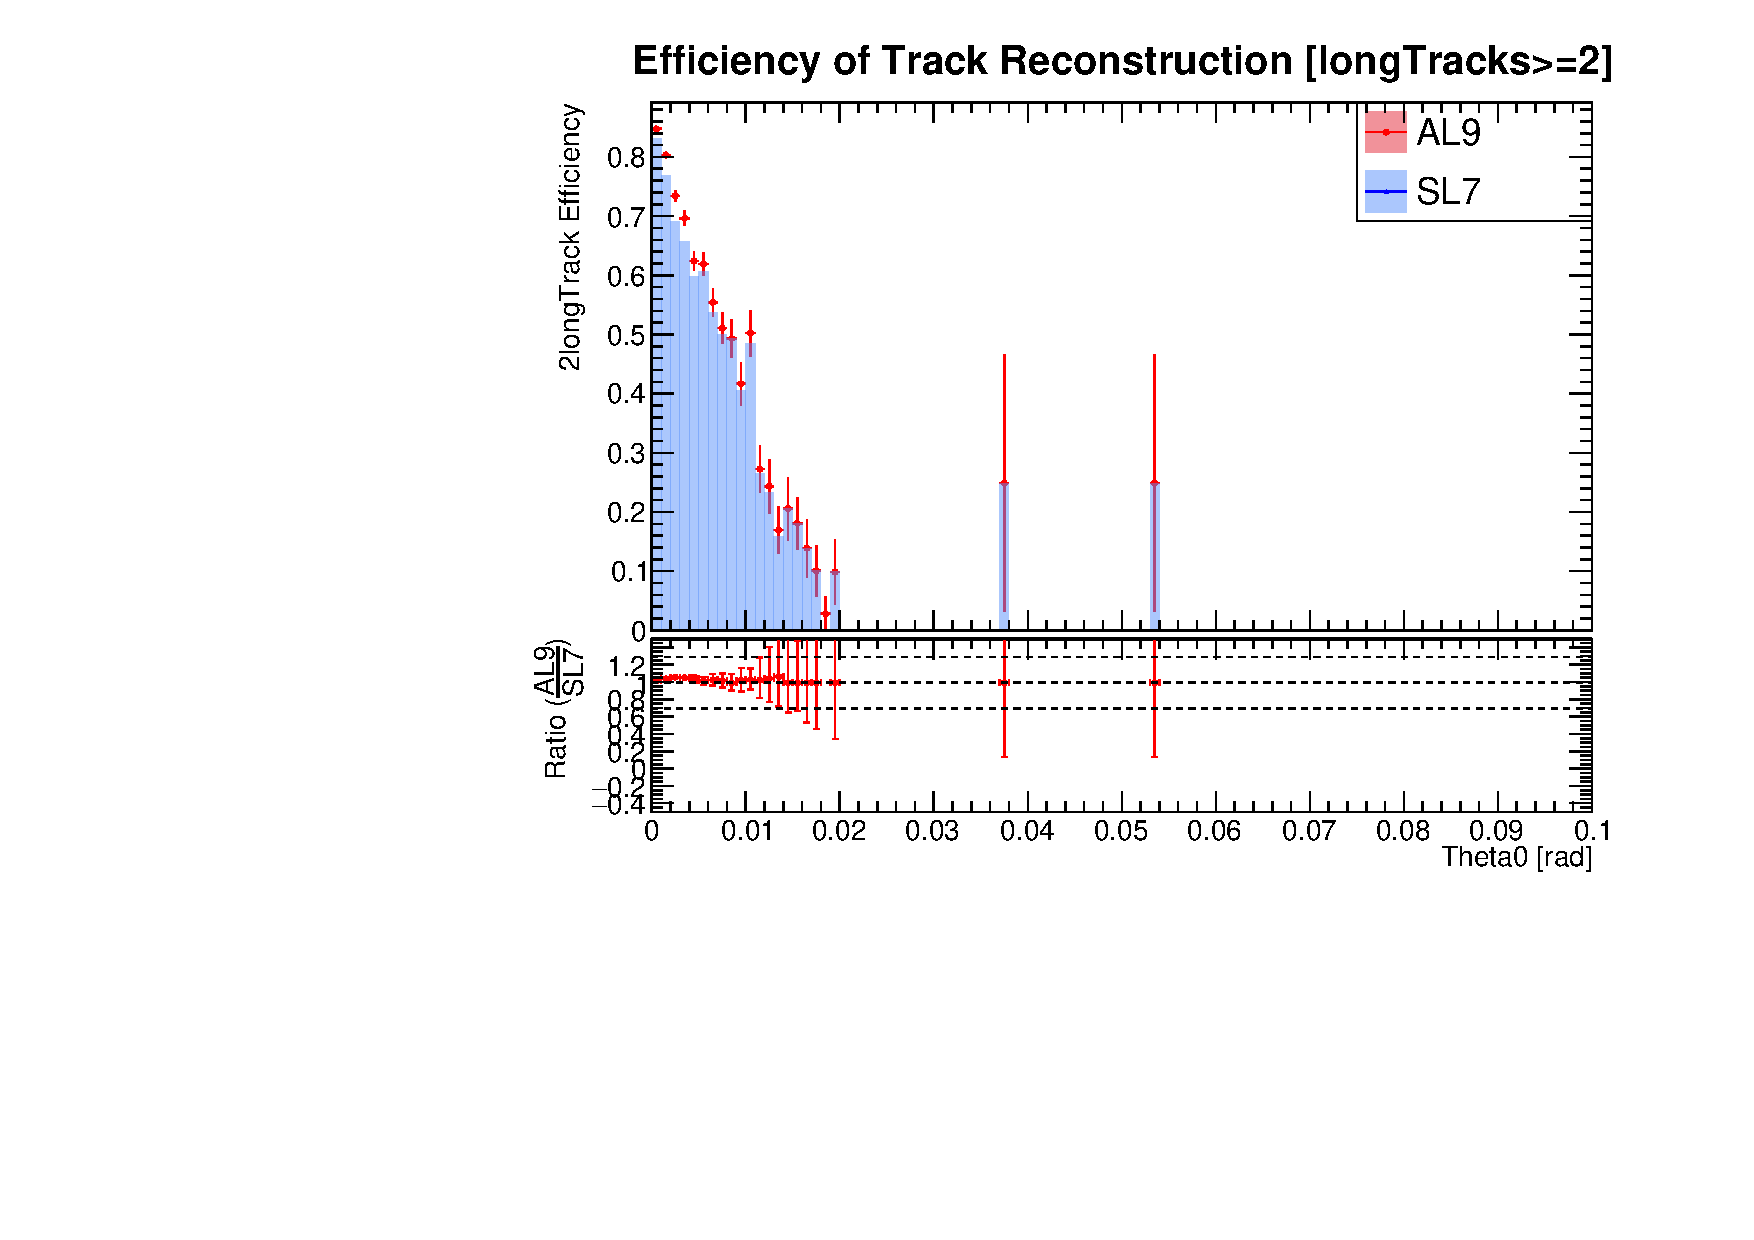
\includegraphics[width=1\linewidth]{./output/Effi_greq2_Theta0.pdf}
            \end{figure}
        \end{column}
    \end{columns}
    \begin{itemize}
        \item The efficiencies at Station 1 seem constant throughout!
        % \item Inconsistent with decay observed from Station 3.
        \item No decrease in efficiency at low separations!
    \end{itemize}
\end{frame}

% \begin{frame}{Comments on $\geq$2 Track Efficiency}
%     \begin{itemize}
%         \item Good agreement between ALMA9 and CENTOS7
%         \item Low statistics at large separation
%         \item The reconstruction is independent of momentum-separation (DeltaRP)
%         \item Efficiencies at Station1 are confusing?
%     \end{itemize}
% \end{frame}



\begin{frame}{Efficiency Metric based on Reconstructed Truth}
    We are interested only in the two primary tracks from $e^+e^-$. Thus we can use the reconstructed truth variables to check if the underlying truth particles are reconstructed.
    \begin{itemize}
        \item For acceptance: Truth Position of $e^+e^-$ $<$ 100
        \item \text{{\textbf{Identify the two primary tracks}} }
        \begin{itemize}
            \item t\_barcode = 2,3 $\implies$ primary tracks 
            \item Also require t\_barcode\_parent = 1 $\implies$ from DarkPhoton
            % \item \lstinline| Any(t_barcode == 2) && Any(t_barcode == 3) && (Sum(t_barcode_parent == 1) >= 2) |

        \end{itemize}
        \item TLDR; Ran the analysis with the above definition, but the results are the exact same as $\geq$ 2 case 
        \item So if event reconstructed has more than 2 longTracks, the two primary tracks are reconstructed, according to above definition.
    \end{itemize}
\end{frame}



\begin{frame}{Efficiency Metric based on Reconstructed Truth}
    \begin{figure}
        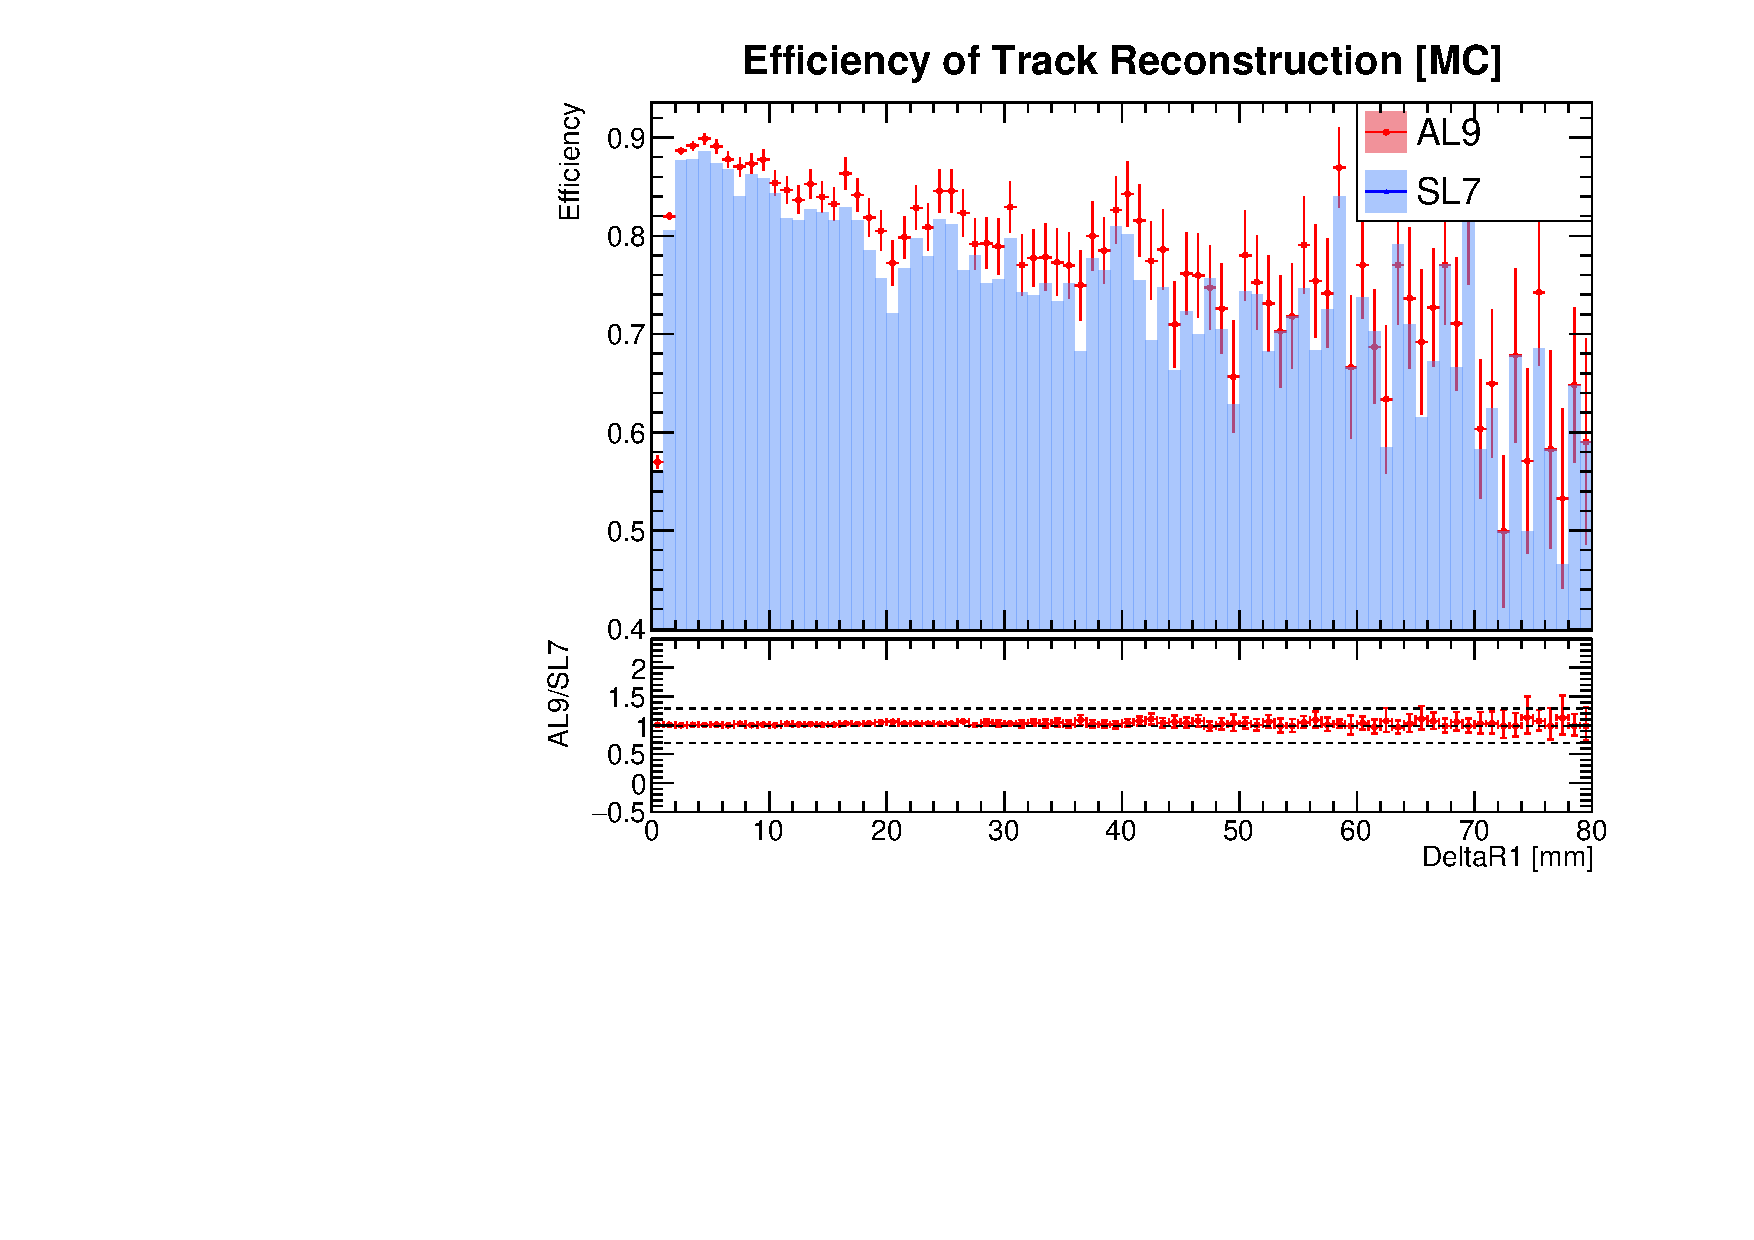
\includegraphics[width=0.9\linewidth]{output/NEffi_MC_pass_DeltaR1.pdf}
        \caption{Efficiency defined using reconstructed truth variables is same as the $\geq$ 2 longTracks definition}
    \end{figure}
    
\end{frame}

\begin{frame}{Conclusions}
    \begin{itemize}
        \small
        \item The ``efficiencies'' generally agrees between ALMA9 and CENTOS7
        \item Lack of agreement with the overlay study
        \item Interpretation of efficiency decay at Station 3 is unclear
        % \item Efficiency at Station 1 is constant, which is inconsistent with Station 3
        \item The resolution of track reconstruction (Track $\chi^2$) has improved.
        \begin{itemize}
            \item Can try to quantify the above in ``efficiency''
        \end{itemize}
        % \item Some differences in ChargeID efficiency
    \end{itemize}
\end{frame}

    
